% === INSERIRE DOPO L'ULTIMA \section{} PRESENTE NEL DOCUMENTO ===

% ============================================================
\section{Alberi Binari di Ricerca}
\label{sec:abr}
% ============================================================

\begin{softnote}
	Gli \textbf{alberi binari di ricerca} (ABR) sono strutture dati che possono essere usate
	come \emph{dizionari} o \emph{code di priorità}. Le operazioni di base hanno costo
	proporzionale all'altezza dell'albero, quindi è importante mantenerli il più possibile
	bilanciati (altezza $\approx \lg n$).
	Quando non è possibile costruire ABR bilanciati si usano varianti come gli
	\textbf{alberi rosso-neri}, che garantiscono altezza $O(\lg n)$ nel caso peggiore.
	Un altro tipo importante sono i \textbf{B-alberi}, adatti a gestire grandi quantità di
	dati nella memoria secondaria (in programma in ``Basi di dati'').
\end{softnote}

% ------------------------------------------------------------
\subsection{Definizione di ABR}
\label{sub:abr_def}
% ------------------------------------------------------------

\begin{definizione}[Albero Binario di Ricerca]
	Un \textbf{albero binario di ricerca} (ABR) è un albero binario in cui ogni nodo $x$
	contiene:
	\begin{itemize}
		\item una chiave $x.\mathit{key}$ (che individua i dati satellite),
		\item i riferimenti $x.\mathit{left}$, $x.\mathit{right}$ e $x.p$ al figlio sinistro,
		destro e al genitore rispettivamente.
	\end{itemize}
	La radice $\mathit{root}$ è l'unico nodo con $x.p = \textsc{null}$.
\end{definizione}

\begin{definizione}[Proprietà fondante]
	Le chiavi in un ABR soddisfano la seguente proprietà. Sia $x$ un nodo:
	\begin{itemize}
		\item se $y$ è un nodo del sottoalbero \textbf{sinistro} di $x$, allora
		$y.\mathit{key} < x.\mathit{key}$;
		\item se $y$ è un nodo del sottoalbero \textbf{destro} di $x$, allora
		$y.\mathit{key} > x.\mathit{key}$.
	\end{itemize}
\end{definizione}

\begin{hardnote}
	La proprietà fondante vale per \emph{tutti} i nodi del sottoalbero, non solo per i figli
	diretti. Lo stesso insieme di chiavi può essere rappresentato da ABR di forma diversa:
	la struttura dipende dall'ordine degli inserimenti.
\end{hardnote}

\begin{definizione}[Albero bilanciato in altezza]
	Un albero binario $T$ è detto \textbf{bilanciato in altezza} (\emph{height-balanced}) se
	\[
	\forall\, t \in T,\quad \bigl|h(t_{\mathrm{sx}}) - h(t_{\mathrm{dx}})\bigr| \leq k,
	\]
	dove $t_{\mathrm{sx}}$ e $t_{\mathrm{dx}}$ sono i sottoalberi sinistro e destro di $t$,
	e $h(t)$ è l'altezza del sottoalbero radicato in $t$. Solitamente $k = 1$.
	In generale, $T$ è detto bilanciato quando la sua altezza è $O(\lg n)$,
	dove $n$ è il numero di nodi.
\end{definizione}

% ------------------------------------------------------------
\subsection{Attraversamento}
\label{sub:abr_attraversamento}
% ------------------------------------------------------------

\subsubsection{Attraversamento Simmetrico (in-order)}
\label{subsub:inorder}

\begin{softnote}
	L'attraversamento \textbf{simmetrico} (in-order) sfrutta la proprietà fondante per
	visitare le chiavi in ordine crescente: si visita ricorsivamente il sottoalbero sinistro,
	poi la radice, poi il sottoalbero destro.
\end{softnote}

\begin{algorithm}[H]
	\caption{\textsc{InOrderTreeWalk}$(x)$}
	\KwIn{Un nodo $x$ di un ABR}
	\If{$x = \textsc{null}$}{\Return}
	\textsc{InOrderTreeWalk}$(x.\mathit{left})$\;
	$\mathrm{visit}(x.\mathit{key})$ \tcp*{visit è una procedura esterna}
	\textsc{InOrderTreeWalk}$(x.\mathit{right})$\;
\end{algorithm}

\begin{nota}
	Su qualunque ABR che rappresenti l'insieme $\{2,5,5,6,7,8\}$,
	\textsc{InOrderTreeWalk} produce sempre l'output ordinato $2,5,5,6,7,8$,
	indipendentemente dalla forma (bilanciata o non) dell'albero.
\end{nota}

\begin{teorema}[Costo di \textsc{InOrderTreeWalk}]
	Se $x$ è la radice di un ABR di $n$ nodi e il tempo di esecuzione di una singola
	chiamata a \emph{visit} è $O(1)$, l'esecuzione di \textsc{InOrderTreeWalk} richiede
	tempo $\Theta(n)$.
\end{teorema}

\begin{proof}
	Sia $T(n)$ il tempo di esecuzione di \textsc{InOrderTreeWalk} su un albero di $n$ nodi.
	\begin{itemize}
		\item $T(n) = \Omega(n)$: banale, si visitano $n$ nodi.
		\item Si deve dimostrare $T(n) = O(n)$.
		\item $T(0) = c$ per il controllo che il nodo sia \textsc{null}.
		\item Per $n > 0$, con il sottoalbero sinistro di $k$ nodi e quello destro
		di $n-k-1$ nodi:
		\[
		T(n) \;\leq\; T(k) + T(n-k-1) + d,
		\]
		dove $d$ è un limite superiore al tempo costante del corpo della chiamata.
		\item Metodo di sostituzione: si assume $T(n) \leq (c+d)n + c$.
		Per $n = 0$ è banale. Per $n > 0$:
		\[
		T(n) \;\leq\; \bigl[(c+d)k + c\bigr] + \bigl[(c+d)(n-k-1) + c\bigr] + d
		\;=\; (c+d)n + c. \qedhere
		\]
	\end{itemize}
\end{proof}

\subsubsection{Pre-ordine e Post-ordine}
\label{subsub:prepost}

Gli attraversamenti in \textbf{pre-ordine} (radice $\to$ sx $\to$ dx) e in
\textbf{post-ordine} (sx $\to$ dx $\to$ radice) non producono una sequenza ordinata
come l'in-order.

\begin{nota}
	Per esercizio: scrivere sia la versione ricorsiva sia quella iterativa di entrambi
	gli attraversamenti.
\end{nota}

% ------------------------------------------------------------
\subsection{Interrogazione di un ABR}
\label{sub:abr_query}
% ------------------------------------------------------------

\begin{softnote}
	Gli ABR supportano le operazioni \textsc{Search}, \textsc{Minimum}, \textsc{Maximum},
	\textsc{Successor} e \textsc{Predecessor}. Ciascuna richiede un tempo $O(h)$, dove $h$
	è l'altezza dell'ABR in input. Per i dettagli si veda~\cite{CLRS}.
\end{softnote}

\subsubsection{Search}
\label{subsub:search}

\begin{algorithm}[H]
	\caption{\textsc{Search}$(x,\, k)$}
	\KwIn{Un nodo $x$ di un ABR, una chiave $k$}
	\KwOut{Un nodo che contiene $k$ se esiste, \textsc{null} altrimenti}
	\If{$x = \textsc{null}$ \textbf{ or } $k = x.\mathit{key}$}{\Return $x$}
	\If{$k < x.\mathit{key}$}{\Return \textsc{Search}$(x.\mathit{left},\, k)$}
	\Return \textsc{Search}$(x.\mathit{right},\, k)$\;
\end{algorithm}

I nodi incontrati durante la ricerca formano un cammino verso il basso dell'albero,
quindi il tempo di esecuzione è $O(h)$.

\begin{esempio}[Ricerca di 13 in un ABR]
	Nell'ABR con radice 15 e nodi $\{2,3,4,6,7,9,13,15,17,18,20\}$,
	la ricerca di 13 esegue il percorso $15 \to 6 \to 7 \to 13$: tre chiamate ricorsive.
\end{esempio}

La versione \textbf{iterativa} è più efficiente in pratica (stessa complessità $O(h)$,
ma costante nascosta minore poiché evita l'overhead dello stack delle chiamate):

\begin{algorithm}[H]
	\caption{\textsc{IterSearch}$(x,\, k)$}
	\KwIn{Un nodo $x$ di un ABR, una chiave $k$}
	\KwOut{Un nodo che contiene $k$ se esiste, \textsc{null} altrimenti}
	\While{$x \neq \textsc{null}$ \KwAnd $k \neq x.\mathit{key}$}{
		$x \leftarrow (k < x.\mathit{key})$ \textbf{ ? } $x.\mathit{left}$ \textbf{ : }
		$x.\mathit{right}$\;
	}
	\Return $x$\;
\end{algorithm}

\subsubsection{Minimum e Maximum}
\label{subsub:minmax}

Per la proprietà fondante:
\begin{itemize}
	\item la chiave \textbf{minima} si trova nel nodo più a sinistra (si scende sempre
	nel figlio sinistro fino a $x.\mathit{left} = \textsc{null}$);
	\item la chiave \textbf{massima} si trova nel nodo più a destra.
\end{itemize}
Entrambe le operazioni hanno costo $O(h)$.

\begin{algorithm}[H]
	\caption{\textsc{Minimum}$(x)$}
	\KwIn{Un nodo $x$ di un ABR}
	\KwOut{Il nodo con la chiave minima nel sottoalbero radicato in $x$}
	\While{$x.\mathit{left} \neq \textsc{null}$}{
		$x \leftarrow x.\mathit{left}$\;
	}
	\Return $x$\;
\end{algorithm}

\begin{nota}
	La procedura \textsc{Maximum} è simmetrica: si scende seguendo i figli destri.
	È lasciata per esercizio.
\end{nota}

\subsubsection{Successor e Predecessor}
\label{subsub:succpred}

\begin{definizione}[Successore]
	Il \textbf{successore} di un nodo $x$ è il nodo con la più piccola chiave $k'$ tale
	che $k' > x.\mathit{key}$ nella sequenza in-order. In un ABR si può trovare senza
	confrontare le chiavi:
	\begin{itemize}
		\item se $x$ ha il sottoalbero destro, il successore è
		\textsc{Minimum}$(x.\mathit{right})$;
		\item altrimenti, è il primo antenato $y$ per il quale $x$ appartiene al sottoalbero
		\emph{sinistro} di $y$ (si risale verso la radice finché si proviene da un
		figlio sinistro).
	\end{itemize}
\end{definizione}

\begin{algorithm}[H]
	\caption{\textsc{Successor}$(x)$}
	\KwIn{Un nodo $x$ di un ABR}
	\KwOut{Il nodo successore di $x$ nella sequenza ordinata dell'ABR}
	\If{$x.\mathit{right} \neq \textsc{null}$}{\Return \textsc{Minimum}$(x.\mathit{right})$}
	$y \leftarrow x.p$\;
	\While{$y \neq \textsc{null}$ \KwAnd $x = y.\mathit{right}$}{
		$x \leftarrow y$\;
		$y \leftarrow y.p$\;
	}
	\Return $y$\;
\end{algorithm}

\begin{nota}
	Nell'ABR di esempio: il successore di 4 è 6, il successore di 13 è 15.
	La procedura \textsc{Predecessor} è simmetrica ed è lasciata per esercizio.
\end{nota}

% ------------------------------------------------------------
\subsection{Inserimento e Cancellazione}
\label{sub:abr_modifica}
% ------------------------------------------------------------

Inserire o cancellare un elemento modifica la struttura dell'albero: occorre sempre
garantire che la nuova struttura soddisfi ancora la proprietà fondante (ripristino).
L'inserimento è semplice; la cancellazione richiede un ripristino più articolato.

\subsubsection{Inserimento}
\label{subsub:insert}

\begin{softnote}
	\textsc{Insert} percorre l'albero dalla radice verso il basso e inserisce $z$ sempre
	come \textbf{foglia} nella posizione corretta. Non controlla la presenza di duplicati:
	può quindi inserire più copie dello stesso valore.
\end{softnote}

\begin{algorithm}[H]
	\caption{\textsc{Insert}$(t,\, z)$}
	\KwIn{Un ABR $t$ e un nodo $z \notin t$
		(con $z.\mathit{left} = z.\mathit{right} = \textsc{null}$)}
	$y \leftarrow \textsc{null}$\;
	$x \leftarrow t.\mathit{root}$\;
	\While{$x \neq \textsc{null}$}{
		$y \leftarrow x$\;
		$x \leftarrow (z.\mathit{key} < x.\mathit{key})$
		\textbf{ ? } $x.\mathit{left}$ \textbf{ : } $x.\mathit{right}$\;
	}
	$z.p \leftarrow y$\;
	\eIf{$y = \textsc{null}$}{
		$t.\mathit{root} \leftarrow z$ \tcp*{$t$ era vuoto}
	}{
		\eIf{$z.\mathit{key} < y.\mathit{key}$}{
			$y.\mathit{left} \leftarrow z$\;
		}{
			$y.\mathit{right} \leftarrow z$\;
		}
	}
\end{algorithm}

\subsubsection{Cancellazione}
\label{subsub:delete}

La cancellazione del nodo $z$ gestisce i seguenti casi:
\begin{enumerate}
	\item $z$ \textbf{non ha figli}: si cancella direttamente $z$.
	\item $z$ \textbf{ha un solo figlio}: il figlio prende il posto di $z$.
	\item $z$ \textbf{ha entrambi i figli} e il suo successore $y$ è figlio diretto di
	$z$ (caso c): $y$ prende semplicemente il posto di $z$.
	\item $z$ \textbf{ha entrambi i figli} e il successore $y$ non è figlio diretto di
	$z$ (caso d): si ricollocano $y$ al posto di $z$ e il figlio destro di $y$
	al posto di $y$. È il caso più complesso.
\end{enumerate}

La soluzione CLRS utilizza la procedura ausiliaria

% === INSERIRE DOPO la descrizione dei casi di cancellazione, PRIMA di Transplant ===

\begin{esempio}[I quattro casi di \textsc{Delete}]
	Consideriamo l'ABR con radice 15 e nodi
	$\{2,3,4,6,7,9,13,15,17,18,20\}$.
	
	\paragraph{Caso (a) — $z$ senza figlio sinistro (es.\ cancella 13).}
	\begin{center}
		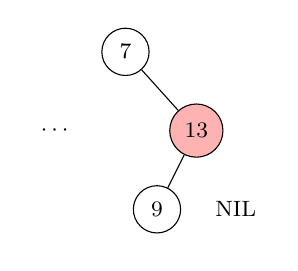
\begin{tikzpicture}[
			every node/.style={circle,draw,minimum size=6mm,font=\footnotesize},
			level distance=10mm, level 1/.style={sibling distance=18mm},
			level 2/.style={sibling distance=10mm}]
			\node {7}
			child{node[draw=none]{$\cdots$} edge from parent[draw=none]}
			child{node[fill=red!30] {13}
				child{node {9}}
				child{node[draw=none]{NIL} edge from parent[draw=none]}
			};
		\end{tikzpicture}
		\quad$\xrightarrow{\text{Delete}(13)}$\quad
		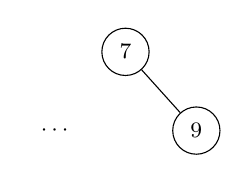
\begin{tikzpicture}[
			every node/.style={circle,draw,minimum size=6mm,font=\footnotesize},
			level distance=10mm, level 1/.style={sibling distance=18mm}]
			\node {7}
			child{node[draw=none]{$\cdots$} edge from parent[draw=none]}
			child{node {9}};
		\end{tikzpicture}
	\end{center}
	\textsc{Transplant}$(t, 13, 9)$: il figlio destro (9) prende il posto di 13.
	
	\paragraph{Caso (c) — entrambi i figli, successore figlio diretto (es.\ cancella 15).}
	Il successore di 15 è 17 (figlio diretto del sottoalbero destro, senza figlio
	sinistro). \textsc{Transplant}$(t, 15, 17)$, poi si aggancia il sottoalbero
	sinistro di 15 come figlio sinistro di 17.
	
	\paragraph{Caso (d) — entrambi i figli, successore non figlio diretto (es.\ cancella 6).}
	Il successore di 6 è 7. Poiché $7.p \neq 6$, prima si esegue
	\textsc{Transplant}$(t, 7, 13)$ (il figlio destro di 7 prende il posto di 7),
	poi \textsc{Transplant}$(t, 6, 7)$ e si riaggancciano i sottoalberi.
\end{esempio}

 \textsc{Transplant}, che sostituisce
il sottoalbero radicato in $u$ con quello radicato in $v$:

\begin{algorithm}[H]
	\caption{\textsc{Transplant}$(t,\, u,\, v)$}
	\KwIn{Un ABR $t$, due nodi $u,v \in t$ ($v$ può essere \textsc{null})}
	\KwOut{In $t$, sostituisce il sottoalbero con radice $u$ con quello con radice $v$}
	\eIf{$u.p = \textsc{null}$}{
		$t.\mathit{root} \leftarrow v$\;
	}{
		\eIf{$u = u.p.\mathit{left}$}{
			$u.p.\mathit{left} \leftarrow v$ \tcp*{$u$ è figlio sinistro}
		}{
			$u.p.\mathit{right} \leftarrow v$\;
		}
	}
	\If{$v \neq \textsc{null}$}{
		$v.p \leftarrow u.p$ \tcp*{Inserisci $v$ in $t$}
	}
\end{algorithm}

\textsc{Transplant} ha complessità $O(1)$.

\begin{algorithm}[H]
	\caption{\textsc{Delete}$(t,\, z)$}
	\KwIn{Un ABR $t$ e un nodo $z \in t$}
	\KwOut{In $t$, cancella $z$ mantenendo $t$ un ABR}
	\If{$z.\mathit{left} = \textsc{null}$}{
		\textsc{Transplant}$(t,\, z,\, z.\mathit{right})$\; \Return \tcp*{caso (a)}
	}
	\If{$z.\mathit{right} = \textsc{null}$}{
		\textsc{Transplant}$(t,\, z,\, z.\mathit{left})$\; \Return \tcp*{caso (b)}
	}
	$y \leftarrow \textsc{Minimum}(z.\mathit{right})$\;
	\If{$y.p \neq z$}{
		\textsc{Transplant}$(t,\, y,\, y.\mathit{right})$
		\tcp*{caso (d): al posto di $y$ metti suo figlio $x$}
		$y.\mathit{right} \leftarrow z.\mathit{right}$
		\tcp*{caso (d): $r$ diventa figlio dx di $y$}
		$y.\mathit{right}.p \leftarrow y$\;
	}
	\textsc{Transplant}$(t,\, z,\, y)$ \tcp*{ultimo passo di (c) e (d)}
	$y.\mathit{left} \leftarrow z.\mathit{left}$\;
	$y.\mathit{left}.p \leftarrow y$\;
\end{algorithm}

\begin{hardnote}
	\textsc{Delete} ha complessità $O(h)$ perché al suo interno può eseguire
	\textsc{Minimum}. Non modificare la struttura prima di aver aggiornato tutti i
	puntatori: l'ordine delle operazioni in \textsc{Delete} è cruciale.
\end{hardnote}

% ------------------------------------------------------------
\subsection{Costruzione di un ABR}
\label{sub:abr_costruzione}
% ------------------------------------------------------------

La complessità delle operazioni fondamentali è $O(h)$. Dalle proprietà degli alberi
binari:
\[
\lfloor \lg n \rfloor \;\leq\; h \;\leq\; n - 1,
\]
dove $n$ è il numero di nodi. Il caso peggiore ($h = n-1$) si raggiunge inserendo le
chiavi in ordine crescente (o decrescente): l'ABR degenera in una lista.

\begin{teorema}[Altezza media di un ABR casuale]
	\label{teo:abr_casuale}
	L'altezza media di un ABR costruito in modo casuale con $n$ chiavi \textbf{distinte}
	è $O(\lg n)$.
\end{teorema}

\begin{nota}
	Un ABR è \emph{costruito in modo casuale} se, partendo dall'albero vuoto, le chiavi
	vengono inserite una alla volta scegliendole casualmente dall'insieme.
	Non sono note formule che stimano l'altezza media dopo una sequenza arbitraria di
	operazioni di inserimento e cancellazione.
\end{nota}

% ------------------------------------------------------------
\subsection{Cenno agli ABR Rosso-Neri}
\label{sub:abr_rn}
% ------------------------------------------------------------

\begin{softnote}
	Operazioni di inserimento e cancellazione possono sbilanciare un ABR fino a renderlo
	degenere. Esistono varianti che mantengono il bilanciamento; la più nota è
	l'\textbf{ABR rosso-nero}.
\end{softnote}

Un ABR rosso-nero associa a ogni nodo un colore (rosso o nero) e rispetta le seguenti
proprietà:
\begin{itemize}
	\item ogni nodo è rosso o nero;
	\item la radice è nera; ogni riferimento a \textsc{null} è considerato nero;
	\item se un nodo è rosso, entrambi i figli sono neri;
	\item per ogni nodo, tutti i cammini semplici dal nodo alle foglie contengono lo
	stesso numero di nodi neri.
\end{itemize}

\begin{teorema}[Altezza degli ABR rosso-neri]
	L'altezza di un ABR rosso-nero con $n$ nodi è al più $2\lg(n+1)$.
\end{teorema}

\begin{hardnote}
	Gli ABR rosso-neri \textbf{non sono in programma} per quest'anno:
	non si richiedono gli algoritmi di inserimento e cancellazione.
\end{hardnote}

% ------------------------------------------------------------
\subsection{Cenno ai Radix Tree}
\label{sub:radix}
% ------------------------------------------------------------

\begin{definizione}[Radix Tree]
	Un \textbf{radix tree} (o \emph{radix trie}, \emph{trie compresso}) è una struttura ad
	albero usata per rappresentare un insieme di stringhe binarie sfruttando i
	\textbf{prefissi comuni}:
	\begin{itemize}
		\item ogni arco è etichettato con un simbolo dell'alfabeto ($0$ oppure $1$);
		\item il cammino dalla radice a un nodo rappresenta il prefisso ottenuto
		concatenando le etichette degli archi attraversati;
		\item una stringa $s$ appartiene all'insieme se esiste un nodo marcato come
		\textbf{terminale} il cui cammino dalla radice è esattamente $s$;
		\item stringhe con prefisso comune condividono la parte iniziale del cammino;
		\item ricerca, inserimento e visita richiedono tempo proporzionale alla lunghezza
		della stringa considerata.
	\end{itemize}
\end{definizione}

\begin{esempio}[Radix tree per $S = \{0,\, 011,\, 10,\, 1001011\}$]
	Le stringhe $0$ e $011$ condividono il prefisso~$0$; le stringhe $10$ e $1001011$
	condividono il prefisso~$10$. I nodi terminali corrispondono esattamente agli elementi
	di~$S$. La struttura ha altezza pari alla lunghezza della stringa più lunga
	dell'insieme (qui: 7).
\end{esempio}

% ------------------------------------------------------------
\subsection{Esercizi}
\label{sub:abr_esercizi}
% ------------------------------------------------------------

\begin{enumerate}
	\item Studiare il Capitolo~12 di~\cite{CLRS}.
	
	\item Dimostrare la correttezza di \textsc{InOrderTreeWalk} per induzione.\\
	\textit{Suggerimento}: la base è un albero con un solo nodo (banale).
	Si suppone che la proprietà valga per alberi di dimensione $n-1$ e si
	considera un albero di $n$ nodi.
	Un albero di $n$ nodi può essere visto come un nodo radice con due
	sottoalberi: uno di $k$ nodi ($0 \leq k \leq n-1$) e uno di $n-1-k$ nodi.
	
	\item Scrivere le versioni ricorsiva \emph{e} iterativa degli attraversamenti in
	pre-ordine e post-ordine.
	
	\item Scrivere la procedura \textsc{Maximum}.
	
	\item Scrivere la procedura \textsc{Predecessor}.
	
	\item Risolvere gli esercizi 12.1-2, 12.1-3, 12.1-4, 12.2-2, 12.2-3, 12.2-4,
	12.2-5, 12.3-1, 12.3-3 di~\cite{CLRS}.\\
	\textit{Suggerimento per 12.1-3}: la soluzione iterativa senza stack richiede
	di trasformare l'albero in un \emph{albero threaded} (con fili).
	Si veda \url{https://www.techiedelight.com/inorder-tree-traversal-iterative-recursive}.
\end{enumerate}